%!TEX program = xelatex
\documentclass[a5paper,12pt,onecolumn]{article}

\usepackage{fontspec}
\setmainfont{Alegreya}
\setmonofont{Inconsolata}
\setsansfont{Averia Sans}

\usepackage[
	papersize={396bp, 596bp},
	ignoreheadfoot,
	total={324bp, 524bp},
	% showframe,
	left = 36bp,
	top = 36bp,
	twoside,
	marginpar = 1in,
	footskip = 2\baselineskip,
]{geometry}

% setup headings
\usepackage{fancyhdr}
\fancypagestyle{plain}{%
	\fancyhf{}
	\fancyfoot[C]{\sf–~\thepage~–}
	\renewcommand\headrulewidth{0pt}
	\renewcommand\footrulewidth{0pt}
}
\pagestyle{plain}

\usepackage{graphicx}
\setkeys{Gin}{width=\linewidth,height=0.915\textheight,keepaspectratio}

\usepackage[final]{listings}
\lstset{
	basicstyle=\footnotesize,
	numbers=left,
	breaklines=true,
	frame=leftline,
	captionpos=b,
	tabsize=2,
	breakatwhitespace=true,
}
\def\code#1{\mbox{\lstinline{#1}}}

\lstnewenvironment{cli}{\lstset{numbers=none, frame=off,}}{}

\usepackage{amsmath}
\usepackage{amsfonts}
\newtheorem{definition}{Definition}

\usepackage{cite}
\usepackage{hyperref}
\usepackage{url}
\usepackage{microtype}
\usepackage{float}

% set the headings
\makeatletter
\renewcommand\section{\@startsection {section}{1}{\z@}%
	{-6.5ex \@plus -1ex \@minus -.2ex}%
	{3.0ex}%
	{\sf\Large}}
\renewcommand\subsection{\@startsection {subsection}{2}{\z@}%
	{-3.5ex \@plus -1ex \@minus -.2ex}%
	{1.5ex}%
	{\sf\large}}
\renewcommand\subsubsection{\@startsection{subsubsection}{3}{\z@}%
	{-5.25ex\@plus -1ex \@minus -.2ex}%
	{1.0ex}%
	{\sf}}
\makeatother

\begin{document}

\begin{center}
	\sf\Huge Seed Tutorial
\end{center}

\section{Prerequisites}

\begin{itemize}
\item Go \url{http://golang.org}
\item Gnuplot
\item Seed \url{https://github.com/nathankerr/seed}
\item A web browser (tested in Safari, Chrome, and Firefox)
\item Some knowledge of command lines, go, javascript, html, and services.
\end{itemize}

\section{Getting Started}

Make a new directory to work in:

\begin{cli}
mkdir seed-tutorial; cd seed-tutorial
\end{cli}

Create a file, \code{kvs.seed}, with the following contents (don't include the line numbers).

\lstinputlisting{start/kvs.seed}

This file defines the core of a key-value store service. Line~1 describes a table called \code{kvstate} with a single key column called \code{key} and a single value column called \code{value}.

Start the service by running:

\begin{cli}
seed -sleep 0.5s -monitor :8000 -execute kvs.seed
\end{cli}

\code{-sleep 0.5s} will sleep half a second in between time steps. This slows things down enough so that we can see what is happening in the service instance. A sleep value is needed when using the monitor to limit the data the web browser must process.

\code{-monitor :8000} starts the debugging monitor on port 8000. To restrict access to localhost, use \code{-monitor localhost:8000}.

\code{-execute} starts the service using the built in interpreter.

The monitor can be accessed at \url{http://localhost:8000} using your favorite web browser:

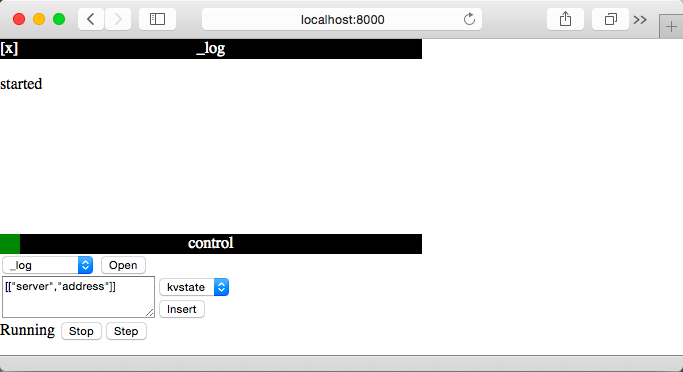
\includegraphics{start/monitor.png}

The debug monitor presents a view of the state of the service instance. The control area has controls for controlling the monitor.

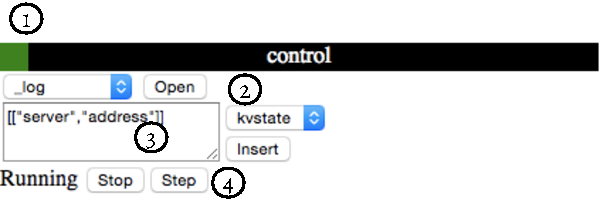
\includegraphics{start/control}

\begin{enumerate}
\item Green shows the monitor is connected; red disconnected.
\item Access to available views. Select the desired view and press open.
\item Insert data into a collection. Data is encoded in JSON as an array of arrays. \code{"server"} and \code{"address"} are special values that are translated into the server and client addresses respectfully.
\item Execution control. Start and stop the service, and step through the parts of the time step.
\end{enumerate}

The rest of the monitor area is for the views. Click on the name of the view to put it in the main area (on the left, where \code{_log} is); \code{[x]} to close the view. Views beginning with underscores are special.

\begin{description}
\item[\_log] The monitor log
\item[\_service] The service that is running (expressed in Seed)
\item[\_graph] The flow graph of the running service. Rule numbers in the graph correspond to those in \code{_service}.
\item[\_time] The time spent on the last timestep
\end{description}

Views not beginning with underscores correspond to collections (e.g., tables, inputs, outputs) in the service.

\section{KVS Put Operation}

\lstinputlisting{put/kvs.seed}

\begin{cli}
seed -sleep 0.5s -monitor :8000 -execute kvs.seed
\end{cli}

Insert stuff into kvput and watch how it flows to kvstate.

\section{Put Client}

The server is the same as the previous section:

\lstinputlisting{client/kvs.seed}

When starting the service, add the network interface by using the \code{networkg} transformation:

\begin{cli}
seed -sleep 0.5s -monitor :8000 -execute -transformations networkg kvs.seed
\end{cli}

The client is a static web page (\code{index.html}):

\lstinputlisting{client/index.html}

Because web browsers don't like allowing websocket access from pages loaded from the local file system, we need a simple web server:

\lstinputlisting{client/server.go}

Start the client web server by:

\begin{cli}
go run server.go
\end{cli}

\section{Replication}

Start the first replica:

\begin{cli}
seed -sleep 0.5s -monitor :8000 -execute -transformations "networkg  replicate" -address :3000 kvs.seed
\end{cli}

Insert \code{[["127.0.0.1:3001"]]} into \code{:8000}'s \code{kvstate_replicants}

Also, set up the views as follows:

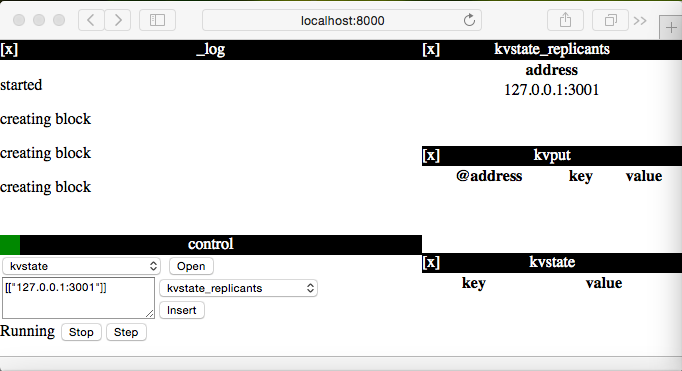
\includegraphics{replicate/first.png}

Start the second replica:

\begin{cli}
seed -sleep 0.5s -monitor :8001 -execute -transformations "networkg  replicate" -address :3001 kvs.seed
\end{cli}

Insert \code{[["127.0.0.1:3000"]]} into \code{:8001}'s \code{kvstate_replicants}

Also, set up the views as follows:

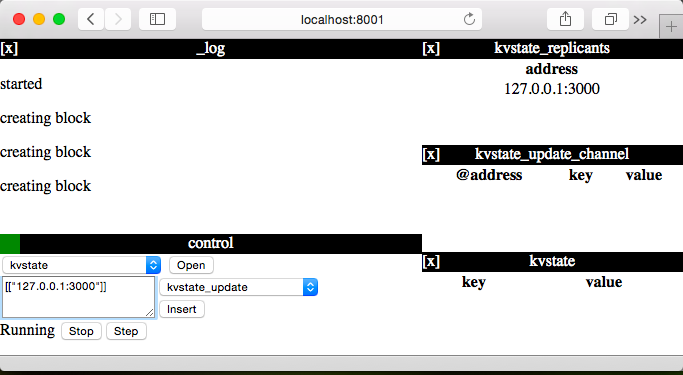
\includegraphics{replicate/second.png}

Start a client (will connect to \code{:3000}):

\begin{cli}
go run server.go
\end{cli}

Put some value into the client and watch as it first hits the first replia and then the second.

Note that due to the transformations, no changes were needed to \code{kvs.seed} or the client to enable replication. However, while the client will only connect to one of the replicas, this could be resolved by using a load balancer.

\end{document}
